\icode{E-MD-MU-L2-261111-001}
如图所示，质量 \(m_1 =\) \,\qty{0.3}{kg}的木板静止在光滑的水平面上，现有质量 \(m_2 =\) \,\qty{0.2}{kg}可视为质点的物块，以水平向右的速度从左端滑上木板，最后在木板上表面某处与木板保持相对静止。物块与木板间的动摩擦因数为 0.5，\(g =\) \,\qty{10}{m/s^2}。则木板的加速度 \(a_1\) 和物块的加速度 \(a_2\) 大小分别为\paren[]

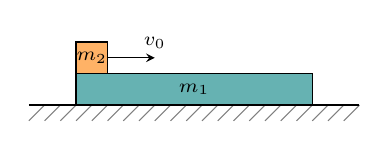
\begin{tikzpicture}[>=stealth,font=\scriptsize]
	\draw[fill=orange!60] (0,.4) rectangle(.4,.8)node[midway]{\(m_2\)};
	\draw[fill=teal!60] (0,0) rectangle(3,.4)node[midway]{\(m_1\)};
	\draw[->] (.4,.6)--++(.6,0)node[above]{\(v_0\)};
	\foreach \x in {-.6,-.4,...,3.6}
		\draw[gray] (\x,-.2)--++(.2,.2);
	\draw[thick] (-.6,0)--(3.6,0);
\end{tikzpicture}
\begin{choices}
	\item \(a_1 = \frac{10}{3}\) \,\qty{}{m/s^2}
	\item \(a_2 =\) \,\qty{5}{m/s^2}
	\item \(a_1 =\) \,\qty{5}{m/s^2}
	\item \(a_2 = \frac{10}{3}\) \,\qty{}{m/s^2}
\end{choices}
\begin{answer}
	AB\qquad 提示：
\end{answer}